% This is "aamas2012 .tex" August 2012 
% This file should be compiled with "aamas2012 .cls" 
% This example file demonstrates the use of the 'aamas2012 .cls'
% LaTeX2e document class file. It is for those submitting
% articles to AAMAS 2012  conference. This file is based on
% the sig-alternate.tex example file.
% The 'sig-alternate.cls' file of ACM will produce a similar-looking,
% albeit, 'tighter' paper resulting in, invariably, fewer pages.
% than the original style ACM style.
%
% ----------------------------------------------------------------------------------------------------------------
% This .tex file (and associated .cls ) produces:
%       1) The Permission Statement
%       2) The Conference (location) Info information
%       3) The Copyright Line with AAMAS data
%       4) NO page numbers
%
% as against the acm_proc_article-sp.cls file which
% DOES NOT produce 1) thru' 3) above.
%
% Using 'aamas2012 .cls' you don't have control
% from within the source .tex file, over both the CopyrightYear
% (defaulted to 200X) and the IFAAMAS Copyright Data
% (defaulted to X-XXXXX-XX-X/XX/XX).
% These information will be overwritten by fixed AAMAS 2012  information
% in the style files - it is NOT as you are used with ACM style files.
%
% ---------------------------------------------------------------------------------------------------------------
% This .tex source is an example which *does* use
% the .bib file (from which the .bbl file % is produced).
% REMEMBER HOWEVER: After having produced the .bbl file,
% and prior to final submission, you *NEED* to 'insert'
% your .bbl file into your source .tex file so as to provide
% ONE 'self-contained' source file.
%

% This is the document class for full camera ready papers and extended abstracts repsectively 

\documentclass{llncs}
\usepackage{amsfonts} % if you want blackboard bold symbols e.g. for real numbers
\usepackage{graphicx} % if you want to include jpeg or pdf pictures
\usepackage{lmodern}
\usepackage{amsmath}
\usepackage{amssymb}
\usepackage{algorithmic}
\usepackage{algorithm}


\usepackage{pgfplots}
\usepackage{filecontents}
\pgfplotsset{compat=newest}



\begin{filecontents}{testdata2.dat}
x whiskerbottom boxbottom median boxtop whiskertop 
1	 149	 4690	 8019	 10907	 142503
2	 105	 1769	 3017	 3807	 58616
3	 98	 141	 317	 544	 82674
4	 111	 17107	 27189	 46238	 403068
5	 145	 3626	 4461	 6126	 119222
6	 63	 463	 707	 913	 44684
7	 64	 3639	 4707	 7416	 189636
\end{filecontents}

\begin{filecontents}{testdata3.dat}
x whiskerbottom boxbottom median boxtop whiskertop 
1 	2329 	4472 	7075 	11553 	78186
2 	469 	2014 	2626 	3623 	49390
3 	78 	143 	378 	428 	42615
4 	382 	10019 	14027 	24771 	189689
5 	1052 	1116 	1218 	1430 	49089
6 	122 	566 	595	643 	30414
7 	153 	1963 	2585 	3596 	67910
\end{filecontents}

\pgfplotsset{
    box plot/.style={
        /pgfplots/.cd,
        black,
        only marks,
        mark=-,
        mark size=\pgfkeysvalueof{/pgfplots/box plot width},
        /pgfplots/error bars/y dir=plus,
        /pgfplots/error bars/y explicit,
        /pgfplots/table/x index=\pgfkeysvalueof{/pgfplots/box plot x index},
    },
    box plot box/.style={
        /pgfplots/error bars/draw error bar/.code 2 args={%
            \draw  ##1 -- ++(\pgfkeysvalueof{/pgfplots/box plot width},0pt) |- ##2 -- ++(-\pgfkeysvalueof{/pgfplots/box plot width},0pt) |- ##1 -- cycle;
        },
        /pgfplots/table/.cd,
        y index=\pgfkeysvalueof{/pgfplots/box plot box top index},
        y error expr={
            \thisrowno{\pgfkeysvalueof{/pgfplots/box plot box bottom index}}
            - \thisrowno{\pgfkeysvalueof{/pgfplots/box plot box top index}}
        },
        /pgfplots/box plot
    },
    box plot top whisker/.style={
        /pgfplots/error bars/draw error bar/.code 2 args={%
            \pgfkeysgetvalue{/pgfplots/error bars/error mark}%
            {\pgfplotserrorbarsmark}%
            \pgfkeysgetvalue{/pgfplots/error bars/error mark options}%
            {\pgfplotserrorbarsmarkopts}%
            \path ##1 -- ##2;
        },
        /pgfplots/table/.cd,
        y index=\pgfkeysvalueof{/pgfplots/box plot whisker top index},
        y error expr={
            \thisrowno{\pgfkeysvalueof{/pgfplots/box plot box top index}}
            - \thisrowno{\pgfkeysvalueof{/pgfplots/box plot whisker top index}}
        },
        /pgfplots/box plot
    },
    box plot bottom whisker/.style={
        /pgfplots/error bars/draw error bar/.code 2 args={%
            \pgfkeysgetvalue{/pgfplots/error bars/error mark}%
            {\pgfplotserrorbarsmark}%
            \pgfkeysgetvalue{/pgfplots/error bars/error mark options}%
            {\pgfplotserrorbarsmarkopts}%
            \path ##1 -- ##2;
        },
        /pgfplots/table/.cd,
        y index=\pgfkeysvalueof{/pgfplots/box plot whisker bottom index},
        y error expr={
            \thisrowno{\pgfkeysvalueof{/pgfplots/box plot box bottom index}}
            - \thisrowno{\pgfkeysvalueof{/pgfplots/box plot whisker bottom index}}
        },
        /pgfplots/box plot
    },
    box plot median/.style={
        /pgfplots/box plot,
        /pgfplots/table/y index=\pgfkeysvalueof{/pgfplots/box plot median index}
    },
    box plot width/.initial=1em,
    box plot x index/.initial=0,
    box plot median index/.initial=1,
    box plot box top index/.initial=2,
    box plot box bottom index/.initial=3,
    box plot whisker top index/.initial=4,
    box plot whisker bottom index/.initial=5,
}

\newcommand{\boxplot}[2][]{
    \addplot [box plot median,#1] table {#2};
    \addplot [forget plot, box plot box,#1] table {#2};
    \addplot [forget plot, box plot top whisker,#1] table {#2};
    \addplot [forget plot, box plot bottom whisker,#1] table {#2};
}


% if you are using PDF LaTex and you cannot find a way for producing
% letter, the following explicit settings may help
 
\pdfpagewidth=8.5truein
\pdfpageheight=11truein

\begin{document}

% In the original styles from ACM, you would have needed to
% add meta-info here. This is not necessary for AAMAS 2012  as
% the complete copyright information is generated by the cls-files.


\title{A Parallel Algorithm for Coalition Structure Generation}

% AUTHORS


% For initial submission, do not give author names, but the
% tracking number, instead, as the review process is blind.

% You need the command \numberofauthors to handle the 'placement
% and alignment' of the authors beneath the title.
%
% For aesthetic reasons, we recommend 'three authors at a time'
% i.e. three 'name/affiliation blocks' be placed beneath the title.
%
% NOTE: You are NOT restricted in how many 'rows' of
% "name/affiliations" may appear. We just ask that you restrict
% the number of 'columns' to three.
%
% Because of the available 'opening page real-estate'
% we ask you to refrain from putting more than six authors
% (two rows with three columns) beneath the article title.
% More than six makes the first-page appear very cluttered indeed.
%
% Use the \alignauthor commands to handle the names
% and affiliations for an 'aesthetic maximum' of six authors.
% Add names, affiliations, addresses for
% the seventh etc. author(s) as the argument for the
% \additionalauthors command.
% These 'additional authors' will be output/set for you
% without further effort on your part as the last section in
% the body of your article BEFORE References or any Appendices.

%\numberofauthors{8} %  in this sample file, there are a *total*
% of EIGHT authors. SIX appear on the 'first-page' (for formatting
% reasons) and the remaining two appear in the \additionalauthors section.
%


% You can go ahead and credit any number of authors here,
% e.g. one 'row of three' or two rows (consisting of one row of three
% and a second row of one, two or three).
%
% The command \alignauthor (no curly braces needed) should
% precede each author name, affiliation/snail-mail address and
% e-mail address. Additionally, tag each line of
% affiliation/address with \affaddr, and tag the
% e-mail address with \email.
% 1st. author
\author{Kim Svensson,\inst{1} Sarvapali D. Ramchurn,\inst{1} Francisco Cruz,\inst{2} Juan-Antonio Rodriguez,\inst{2} Jesus Cerquides\inst{2}}
\institute{Electronics and Computer Science, University of Southampton, SO17 1BJ, UK
\email{\tt\{ks,sdr\}@ecs.soton.ac.uk} 
\and
IIIA, CSIC, Spain
 \email{\tt\{tito,jar,jesus\}@iiia.csic.es}
}

\maketitle

\begin{abstract}
We develop the first parallel algorithm for combinatorial optimisation problem of Coalition Structure Generation (CSG) that is central to many multi-agent systems applications. Our approach involves distributing the key steps of a dynamic programming approach to CSG across computational nodes on a Graphics Processing Unit (GPU) such that each of the thousands of threads of computation can be used to perform small computations that speed up the overall process. In so doing, we solve important challenges that arise in solving combinatorial optimisation problems on GPUs such as the efficient allocation of memory and computational threads to every step of the algorithm. In our empirical evaluations on a standard GPU,  our results show an improvement of orders of magnitude over current dynamic programming approaches with an ever increasing divergence between the CPU and GPU-based algorithms in terms of growth. Thus, our algorithm is able to solve the CSG problem for 29 agents in one hour as opposed to two days for the current state of the art dynamic programming algorithms.
\end{abstract}

% Note that the category section should be completed after reference to the ACM Computing Classification Scheme available at
% http://www.acm.org/about/class/1998/.

%\category{H.4}{Information Systems Applications}{Miscellaneous}

%A category including the fourth, optional field follows...
%\category{D.2.8}{Software Engineering}{Metrics}[complexity measures, performance measures]

%General terms should be selected from the following 16 terms: Algorithms, Management, Measurement, Documentation, Performance, Design, Economics, Reliability, Experimentation, Security, Human Factors, Standardization, Languages, Theory, Legal Aspects, Verification.

%\terms{Delphi theory}

%Keywords are your own choice of terms you would like the paper to be indexed by.

%\keywords{AAMAS proceedings, \LaTeX, text tagging}

\section{Introduction}
\noindent Coalition formation is a one of the key coordination mechanisms in
multi-agent systems. It involves the coming together of a number of  agents to
achieve some individual or group objective.  An important step in the 
 coalition formation process involves partitioning the set of agents into coalitions that, on aggregate (as a coalition structure), maximise the efficiency in the system. This problem is termed the 
\emph{Coalition Structure Generation} problem (CSG)
~\cite{DBLP:journals/ai/SandholmLAST99}.   The  CSG problem is a hard combinatorial optimisation problem and scales in $\omega(n^n)$ \cite{DBLP:journals/ai/SandholmLAST99}. To date, many algorithms have been designed to solve the CSG. These range from branch-and-bound approaches such as \cite{rahwan2009anytime}, to dynamic programming approaches such as
\cite{DBLP:conf/atal/RahwanJ08,rahwan:jennings:2008b}. The latter are particularly attractive given their lower complexity but most of these algorithms scale to around 30 agents given the exponential growth in computation involved. We also note that these algorithms were mainly designed for single threaded architectures, and even if distributed variants exist \cite{distcsg}, these require storing the input data redundantly across multiple computers and sharing information over network links that may be liable to delays and losses. 

In contrast, in the last few years, a surge in the development of frameworks for parallel programming on a single machine has been noted with the development of general purpose Graphics Processing Units (GPUs). Indeed, these processors, originally developed for only processing high end graphics, can now be programmed to perform simple mathematical operations that, when performed in thousands in parallel, can significantly outperform single-threaded machines with higher frequencies and memory speeds. There are multiple challenges, however, that need to be overcome before complex algorithms as for CSG can be implemented onto the GPU (we elaborate on these in Section \textbf{XX}) including the need to limit random memory access,  the limits on the number of threads that can be launched to share the same memory blocks, and the need to avoid loading data frequently from main memory. 

Against this background, in this paper, we present a parallel algorithm for CSG for highly multi-threaded GPUs that meets the challenges above and outperforms the best algorithms for CSG. Our algorithm, GPU-CSG, parallelises the computation of individual steps of a dynamic program to solve the CSG. It does so by partitioning the computation across thousands of threads where each solves a small sub-problem of the larger optimisation problem. The solution to each sub-problem is then used to find the best partition of agents. In more detail, this paper advances the state of the art in the following ways. First, we develop the first parallel  algorithm for CSG that avoids redundant memory storage and inter-processor communication. Second, we prove that GPU-CSG is correct and complete and demonstrate through empirical evaluation that its growth rate is significantly lower than that of the dynamic programming approach it builds upon. Third, we empirically show that GPU-CSG outperforms the state of the art by orders of magnitude, solving the CSG problem for 30 agents in \textbf{XX} hours as opposed to \textbf{XX days or months} for the previous state of the art.

The rest of this paper is structured as follows. Section 2 presents the
background to this work and discusses related work while Section 3 introduces
the GPU architecture. Section 4 then details the DP algorithm upon which we build GPU-CSG
while section 5 while Section 7 concludes.

\section{Background}

\subsection{Coalition formation}


\subsection{The {DP} Algorithm} 
%done


The DP algorithm as shown in algorithm \ref{DP} works by producing two output tables, $O$ and $f$, 
where each table have one entry per coalition structure. 
An entry in $f$ represent a value a certain coalition structure is given, 
while $O$ represent which splitting, if any, maximised the coalition structure for the entry in $f$ which it represent.
More elaborated, given all coalitions of agents $C\subseteq A$, for each coalition in $C$, evaluate all
pairwise disjoint subsets here named splittings on their pairwise collective sum against the coalitions
original value. Given one splitting is greater, update the value of the coalition $f(C) := f(C') + f(C\setminus C')$
and assign $O$ on $C$ to represent the new splitting, $O(C) := \{C',C\setminus C'\}$. These steps are first carried out
on all coalition structures with two agents, continuing until $N$ agents. 
This means, given a coalition structure $S$ with cardinality $|S| = n$, then all coalition structures
for the sizes 1,2,...,n-1 have already been evaluated. The dynamic programming algorithm is entirely deterministic meaning
that even if there was only one or two valuations, the algorithm will evaluate all splittings before it reaches a conclusion.
However this algorithm does not work well with an large amount of agents as it grow exponential and have an time complexity of $O(3^n)$.
As described later in section ?? the part of the algorithm that is paralleled is the max function on line \ref{lst:line:a}
which handles the evaluation of all splittings of a given coalition structure.

\begin{algorithm}
\caption{Dynamic Programming algorithm \label{DP}}
INPUT: $b$: collection of the bids for all coalitions\\*
VARIABLES: $f$: collection holding the maximum value for all coalitions\\*
$O$: collection holding the most beneficial splitting for all coalitions.
\begin{algorithmic}[1]
\STATE\algorithmicfor\ all $x \in A$, \algorithmicdo  $f(\{x\}):= b(\{x\}),O\{x\}:= \{x\}$ \algorithmicendfor
\FOR{$i := 2$ to $n$}
\FOR{all $C \subseteq A: \vert C \vert == i$}
\STATE $f(C) := max\{f(C\backslash C')+f(C'):C'\subseteq C \wedge 1 \leq \vert C' \vert \leq \dfrac{\vert C \vert}{2}\}$ \label{lst:line:a}
\STATE\algorithmicif $f(C) \geq b(C)$ \algorithmicthen\ $O(C) := C^{*}$ \hfill Where $C^{*}$ maximizes right hand side of line~\ref{lst:line:a} \algorithmicendif
\STATE\algorithmicif $f(C) < b(C)$ \algorithmicthen\ $f(C) := b(C)\wedge O(C) := C$ \algorithmicendif
\ENDFOR
\ENDFOR
\STATE Set $CS^* := \{A\}$
\FOR{all $C \in CS^*$} \label{lst:line:redo}
\IF{$O(C) \neq C$}
\STATE Set $CS^* := (CS^*\setminus \{C\})\cup \{O(C),C\setminus O(C)\}$ 
\STATE Goto \ref{lst:line:redo} and start with a new $CS^*$
\ENDIF
\ENDFOR
\RETURN $CS^*$
\end{algorithmic}
\end{algorithm}

The table $O$ may be discarded and not calculated to reduce the memory requirement by half removing instant access to the final splittings.
These final splittings are easily retrieved as outlined in algorithm \ref{idpref}. 
Essentially, all coalitions in $C \in CS^*$ which value in $f$
is not equal to the initial bid in $b$, find the first splitting that is equal to the value in $f$.
The overhead of this is insignificant as it needs to evaluate at most $n -1$ coalitions compared to the exponential
number of evaluations carried out in the previous steps\cite{eps265062}.

\begin{algorithm}
\caption{Enumeration of the optimal splittings through re-evaluation of small amount of coalitions \label{idpref}}
INPUT: $b:$ array of the initial bids for all coalitions $C \subseteq A$. 
$f:$ the final evaluated values gathered from evaluating splittings.
\begin{algorithmic}[1]
\STATE Set $CS^* := \{A\}$
\FOR{all $C \in CS^*$} \label{lst:line:redo2}
\IF{$f(C) \neq b(C)$}
\STATE find first $C^*$ where $f(C) = f(C\backslash C^*)+f(C^*):C^*\subseteq C \wedge 1 \leq \vert C^* \vert \leq \dfrac{\vert C \vert}{2}$ \label{lst:line:aa}
\STATE Set $CS^* := (CS^*\setminus \{C\})\cup \{C^*,C\setminus C^*\}$
\STATE Goto \ref{lst:line:redo2} and start with a new $CS^*$
\ENDIF
\ENDFOR
\RETURN $CS^*$
\end{algorithmic}
\end{algorithm}



\subsection{The CUDA Architecture} %done
Graphics Processing Units(GPU) from NVIDIA and AMD is highly multi-threaded, many-core architectures primarily aimed at 
highly parallel image processing and rendering, however it have in the recent years moved towards supporting general purpose computing through 
the OpenCL and NVIDIA CUDA framework.
It does so by devoting a larger amount of transistors towards many computational units rather than data caching and advanced 
flow control more often seen in CPU architectures.
NVIDIA describes their general purpose GPU CUDA architecture as a Single Instruction Multiple Threads (SIMT) architecture, 
meaning groups of multiple threads execute the same instructions concurrently and is proportional to SIMD architectures. 
This enables their GPUs to be highly advantageous when performing data-independent and non-divergent tasks.
To understand this further the grouping of the threads need to be explained and is outlined in figure \ref{fig:reduction}.
A kernel which is a device specific CUDA function that is called by the sequential host code,
will request a specified number of blocks in a grid of blocks.
Each block may to this date consist of up to 1024 threads depending on the compatibility of the card, with a maximum
grid size of $2^{31}-1$ blocks subjected to compatibility. When run, the blocks will be distributed onto available multiprocessors,
which then independently schedule the run-time of the block. Note that blocks may be executed concurrently or sequential depending on
the current workload and the number of available multiprocessors.
The block is split into smaller units of 32 threads called warps, all threads within the same warp are always scheduled
the same instruction to be run and this is what embodies the SIMT paradigm. 
Therefore, branching threads causing inter-warp divergence means a warp will have inactive threads not executing any instructions, 
which may lead to poor efficiency with worst case of sequential performance. Further, warps are scheduled independently of each other
meaning possible concurrent execution of warps.

The threads communicate with each other through writes to various types of memory outlined in table \ref{mem}.
There are three types of thread writable memory in the architecture; registers and local memory are each threads
coupled memory which is not volatile and may be shared with other threads inside the same warp as described in section \ref{reduction}. 
Shared memory is as its name tells shared between all threads within the same block, as it may be written to by any thread within the block
it should be treated as volatile, thus synchronization inside the block have to be consider whilst dealing with shared memory.
Finally, global memory is the only persistent memory which will persist between each kernel call, it may be manipulated by the host,
but also by any thread, and is the only means of communication in between kernels, blocks, and the host. It to should be considered volatile.

Regarding access to the global memory, certain access patterns must be followed in order maximise performance. 
For global memory, it is important to note that each load request from memory will fetch in cachelines of size $32*wordsize$,
meaning cachelines of 32, 64, and 128 bytes each when pulling the primitives char, short and int respectively.
The reason for this is the fact mentioned earlier, all 32 threads within the same warp issue the same instruction, 
thus each warp fetches 32 entities of a specific word type.
As a result, if the memory reads within a warp is not coalesced(grouped within the same cacheline) within consecutive words, the effective bandwidth will drop immediately.

\begin{table}
\centering
\caption{Memory scope, lifetime, and speed \label{mem}}
\begin{tabular}{|l|l|l|l|} \hline
Type&Scope&Lifetime&Relative Speed \\ \hline
Register&Thread \& Warp&Thread&Fastest\\
Shared&Block&Block&Fast\\
Global&Kernel \& Host&Program&Slow\\
\hline\end{tabular}
\end{table}

\subsection{Data structure} %done
How the data is represented and structured is important, 
especially in bandwidth bound algorithms where the majority of time
is spent fetching data from memory and the arithmetic overhead is low.
Selecting the right composition will reduce the memory requirements substantially.
Given the two entities of data that is needed to be represented for each coalition structure, 
the coalition structure itself and its value in $f$. 
Memory constraints will be imposed given a large amount of agents as a result of DP's exponential growth.

In order to minimize memory usage several techniques were used. 
Representing a coalition structures members as an array of values,
where each value represent a distinct agent may seem intuitive at first. 
However, if the members are represented as bits set in a fixed sized integer, the memory
requirement will be reduced substantially as shown by previous studies.\cite{boyer2012solving}
If solving for the complete coalition structure formation problem with n agents representing members as an array of values.
There are \begin{math}\dbinom{n}{i}\end{math} coalition structures of size $i$, where
$i$ entries have to be stored per coalition structure.
The total number of values needed to store just to represent the coalition structures is there for equal to:
\begin{displaymath}\sum_{i=i}^{n} \dbinom{n}{i}*i\end{displaymath}

Given the same constraints, representing the coalition structure as an fixed sized integer, it is only 
needed to store one entry per coalition structure, totaling to \begin{math}2^n-1\end{math} data points.

To give an example, with four agents $A = {f_0,f_1,f_2,f_3}$, the coalition $C = {f_0,f_2,f_3}$ would be represented
as $C = 1101$ in the binary system and $13$ in the decimal system. Therefore, if the coalition
structure is represented as an integer it can implicitly be stored as an index 
to its coalition value, by enumerating it on run-time. That means the only
memory constraint on the system is the store all the values for all the coalition structures.

\subsubsection{Coalition Structure Splittings}

\begin{table}
\centering
\caption{Splittings of $C = \{f_0,f_2,f_3\}$ Binary $C = 1101$ \label{split}}
\begin{tabular}{|l|c|c|c|} \hline
Set& $\{f_0\}$\hfill$\{f_2,f_3\}$ &$\{f_2\},\{f_0,f_3\}$&$\{f_3\},\{f_0,f_2\}$ \\ 
system&&& \\ \hline	
Binary&0001\hfill 1100&0100\hfill 1001&1000\hfill 0101 \\
system&&& \\
\hline\end{tabular}
\end{table}


\begin{table}
\centering
\caption{Initialize shift on $C = \{f_0,f_2,f_3\}$\label{split}}
\begin{tabular}{|l|r|r|} \hline
Binary&$1_3 1_2 0_1 1_0$&\\ \hline
Shift&\vline 0\vline 3\vline 2\vline 0\vline& Result \\ \hline
Splitting 1 & $0001 : 1 << shift[0]$& $0001$ \\ 
Splitting 2 & $0010 : 1 << shift[1]$&$ 0100$ \\
Splitting 3 & $0011 : 1 << shift[0]$&\\ & $+ 1 << shift[1]$&$0101$ \\
\hline\end{tabular}
\end{table}

\begin{algorithm}
\caption{initShift input $Coalition:C$ \label{initshift}}
\begin{algorithmic}[1]
\STATE $t :=C$
\STATE $count := 0$
\WHILE{$t > 0$} {
\STATE $index := FindFirstSet(t)$
\STATE $shift_{count} := index$
\STATE $nullBit(t,index)$
\STATE $count++$
}
\ENDWHILE
\RETURN shift
\end{algorithmic}
\end{algorithm}



Splittings as mentioned are pairwise disjoint subsets of a coalition structure, 
given the coalition structure $C = \{f_0,f_3,f_4\}$ the splittings
are shown in table \ref{split}. In order to generate the splitting there is essentially two methods used, 
the, initShift, initialSplit and nextSplit methods. 
The function initShift as detailed in algorithm \ref{initshift} is necessary to setup the environment for 
all calls to initialSplit, what it does is using the bit operation $find first set$ to find the indexes of all bits set
in from the integer coalition input. This will give each entry in the $shift$ array an unique number. 
This unique numbers will be used by initialSplit to distribute the bits of the count to fit the configurations bits.
It does so by taking a count as input representing which nth splitting should be created, finds the index of its 
set bits, and finally left shifts each bit with the value in the shift array its index reference to.

nextSplit works through a recurrence relation which means in order to have 
concurrent threads independent of each other, an initial splitting for each thread have to be calculated using initialSplit. 
initialSplit works by first generating an packed index array of which bits are set in the coalition structure using initShift.
Given which nth splitting it should generate, it distributes the bits of $n$ to the corresponding bits of coalition $C$. 
Thereafter nextSplit will be used to generate the next splitting. 


\begin{algorithm}
\caption{ nextSplit input $Coalition:C$ $Splitting:S$}
\begin{algorithmic}[1]
\STATE $C' := twosComplement(C)$
\STATE $S' := bitwiseAND((C'+S),C)$
\RETURN $S'$
\end{algorithmic}
\end{algorithm}

\begin{algorithm}
\caption{initialSplit input $Count:n, Coalition:C$}
\begin{algorithmic}[1]
\STATE $t := n$
\STATE $S := 0$
\WHILE{$t > 0$} {
\STATE $index := FindFirstSet(t)$
\STATE $S := S + leftShift(1,shift_{index,C})$
\STATE $nullBit(t,index)$??
}
\ENDWHILE
\RETURN $S$
\end{algorithmic}
\end{algorithm}

\begin{algorithm}
\caption{Fetch using Collision detection \label{collision}}
Input:
Index:$\psi$ \hfill Which nth splitting should be generated
Index:$z$ \hfill The index in $\upsilon$ for the coalition structure that is evaluated 

Variables:Value $\alpha $: \hfill Holds temporary values

\begin{algorithmic}[1]
    \STATE $C_{0} := initialSplit(\psi,CS_0)$ \label{lst:line:startcol}
    \STATE $C_{1} := initialSplit(\psi,CS_1)$
    \STATE $\upsilon_{0,z} := f(C_{0})$ \label{lst:line:fetch}
    
    \IF{$C_{1} = C_{0}$} \label{lst:line:firstif}
      \STATE $\upsilon_{0,z+1} := \upsilon_{0,z}$
      \ELSE
      \STATE $\upsilon_{0,z+1} := f(C_{1})$
     \ENDIF \label{lst:line:firstifend}
    \STATE $C_{0} := CS_0\backslash C_{0}$ \label{lst:line:startend}
    \STATE $\alpha := f(C_{0})$
    \STATE $C_{1} := CS_1\backslash C_{1}$
    \IF{$C_{1} = C_{0}$}
      \STATE $\upsilon_{0,z+1} := \upsilon_{0,z+1}  + \alpha$
    \ELSE
      \STATE $\upsilon_{0,z+1} := \upsilon_{0,z+1} + f(C_{1})$
    \ENDIF
    \STATE $\upsilon_{0,z} := \upsilon_{0,z}  + \alpha$ \label{lst:line:endend}
\RETURN $\upsilon$
\end{algorithmic}
\end{algorithm}
\subsubsection{Collisions between Splittings of Coalitions} \label{sectionsplit}
Given that each thread evaluate several splittings over numerous coalition structures in parallel, 
it is bound that splittings on two coalition structures that overlap will have splittings that collide.
A collision means that splittings of coalition structures contain at least one identical subset shared between them.
\begin{displaymath}\forall S\subset C \wedge S' \subset C' : C \cap C' \neq \emptyset \Rightarrow \exists S \wedge S' : S = S'\end{displaymath}
For all splittings of $C$ and $C'$ where the coalition structures intersect, there must exist at least one splitting shared between them.

The number of splittings that collide is dependent on how many common members the coalitions have in common.
\begin{displaymath}2^{n-1}-1:C\neq C'\wedge |C \cap C'| = n \wedge n > 1 \end{displaymath}
Specifically, the number of splittings in common is how many splittings
can be done all the members in common.
Normally, each splitting would be fetched from global memory resulting in it being fetched several times, 
if it have not been evicted from the cache memory.

By using collision detection as described in algorithm \ref{collision} the number of redundant fetches may be reduced.
It works by evaluating two or more coalitions at the same time, lines \ref{lst:line:startcol} to \ref{lst:line:fetch} generates
the initial splittings and fetches the value for the first splitting. It then trough lines \ref{lst:line:firstif} to \ref{lst:line:firstifend}
checks whether the splitting of the second splitting is equal to the first. 
If so assign it the first splittings value, else fetch its own value from global memory. 
Finally, the last lines does the same thing as above just that it does that on the pairwise disjoint subset, 
and the first splittings next value is stored in an temporary variable. 
The more splittings that are evaluated at the same time and checked against each other, the less redundant memory fetches are done.


\subsubsection{Reduction} \label{reduction} %done
\begin{figure*}
\centering
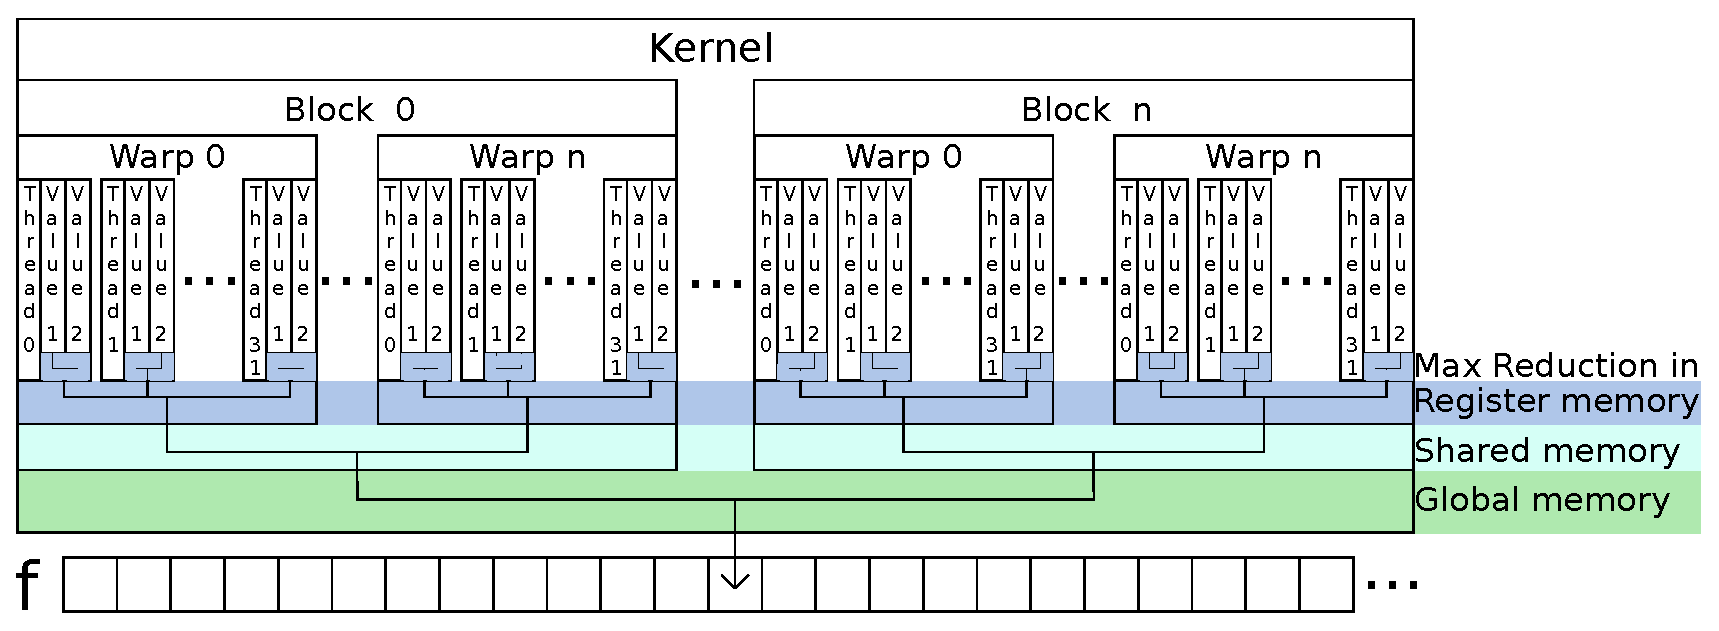
\includegraphics[width=\linewidth]{reduction}
\caption{Outline of reduction across thread, warp, block and kernel \label{fig:reduction}}
\end{figure*}

As the evaluation of each coalition structure is to find the splitting 
of the coalition structure which maximizes the value of the coalition structure,
it is simply needed to compare the values of all splittings with each other to find the most valued one. 
The reduction is done on four levels of scope as seen on lines \ref{lst:line:reductionstart} to \ref{lst:line:reductionend} in algorithm \ref{gpudp},
as well as outlined in figure \ref{fig:reduction}. 

On thread level, each thread evaluate a number of splittings to determine their most valued splitting. 
On warp level, all threads inside the same warp concurrently exchange their largest register values to find the most valued splitting among the warp.
This is done by utilizing a function called $\_\_shfl\_xor$ which allows for an exchange of register values between any thread within the same warp.
Using this technique allows for a substantial reduction in shared memory use, as all that is needed to be stored is one value per warp in shared memory. 
With each single value from each warp moved into shared memory, initially the total number of active threads will be equal to the number
of warps inside the block divided by two. These thread will compare one warp value each with the respective value that is not being compared by
another thread, half the number of threads and iterate over again. This is done until only one thread remains which will compare the last two values.
Finally, the single thread that compared the last values, will try to update the value in global memory if it is larger using atomic functions.

\subsection{Algorithm} %not done nein
The algorithm starts by initializing all the variables needed further on,
as generating the next coalition structure works through a recurrence relation, 
only the first thread will update the shared memory. Continuing, next step is to generate the shift array, 
this can be done in parallel so a number of threads invoke the method initShift.
\begin{algorithm}
\caption{GPU implementation of the DP algorithm\label{gpudp}}
\textbf{Input}

$f$\hfill The array which holds the bids

$C_0$\hfill The first coalition structure to do evaluation on

$\Psi$\hfill The maximum number of splittings

\textbf{Constants}

$\lambda$ \hfill How many bids should be evaluated per thread

$confpkernel$

$nparallelconf$

\textbf{Variables} 

$\Upsilon$ \hfill A shared array containing warps maximum bid values

$\upsilon$ \hfill A local array containing one of the threads bid value

$bid = blockIdx.x$ \hfill Which block the threads belong to

$conf$

$bdim = blockdim.x$ \hfill How many threads inside the block

$tid = threadIdx.x$ \hfill The thread index inside the block

$\psi := \lambda*(tid+bdim*bid)$ \hfill Initial subset construction index

\textbf{Start of algorithm}
\begin{algorithmic}[1]
\IF{$tid = 0$}
  \STATE $conf_0 := C_0$
  \FOR {$i := 1$ to $confpkernel$}
    \STATE $conf_i := nextCoalition(conf_{i-1})$
  \ENDFOR \hfill Checkpoint 1
\ENDIF
\IF{$tid < confpkernel$}
  \STATE $initShift(conf_{tid})$ 
\ENDIF
\hfill Checkpoint 2
\FOR{$x := 0$ to $confpkernel$}
  \STATE Set all values in $\upsilon$ to 0

  \IF{$\psi \geq \Psi$}
    \STATE goto postfetch
  \ENDIF
\hfill Checkpoint 3
  \FOR{$z := 0$ to $nparallelconf$}
    \IF{$conf_{z+x} \geq maxval$}
      \STATE break
    \ENDIF
    \STATE $C_z := initialSplit(\psi,conf_{z+x})$
    \STATE $\upsilon_{0,z} := f(conf_{z+x}\backslash C_z)+f(C_z)$
    \STATE $C_z := nextSplit(C_z)$
    \STATE $\upsilon_{1,z} := f(conf_{z+x}\backslash C_z)+f(C_z)$
    \STATE $z := z + 2$
  \ENDFOR
\hfill Checkpoint 4
  \FOR{$z:=0 to nparallelconf$}\label{lst:line:reductionstart}
  
    \IF{$\upsilon_{1,z} > \upsilon_{0,z}$}
      \STATE $\upsilon_{0,z} := \upsilon_{1,z}$
    \ENDIF
    
    \STATE $warpReduction(\upsilon_{0,z})$

    \IF{$tid \% 32 = 0$}
      \STATE $i := tid / 32$
      \STATE $\Upsilon_{i,z} := \upsilon_{0,z}$
    \ENDIF
  \ENDFOR   \hfill Checkpoint 5
  \STATE $blockReduction()$
  \hfill Checkpoint 6
  \IF{$tid = 0$}
  \STATE $atomicUpdate()$\label{lst:line:reductionend} 
  \ENDIF  \hfill Checkpoint 7
  \STATE $x := x + nparallelconf$
\ENDFOR
\end{algorithmic}
\end{algorithm}

\subsection{Experimental setup}

The GPU instance of the algorithm was run on a Linux desktop computer using CUDA version 5.0 containing 12GiB DDR3 RAM, 
3.2GHz AMD Phenom II X4 CPU and a consumer grade NVIDIA GeForce GTX 660 Ti with a GPU clock of 915MHz and 6008MHz effective clock on the memory.
It ran 256 threads per block, with each thread evaluating two splittings per coalition structure, 
where 8 coalition structures was evaluated in parallel for a total of 32 coalition structures visited.
The CPU DP algorithm is run single threaded on a INTEL XEON W3520 with a clock-speed of 2.67GHz with 32KB L1, 256KB L2 cache. 
The way the data is structured and stored is identical between both implementations.
\section{Results}

%\begin{figure}[width=\linewidth]
%\caption{LOG Clock Cycles between checkpoints and relative time for each code segment, not sharing splittings\label{nosplitt}}
%\begin{tikzpicture}[align=left]
%\begin{axis} [
%%scale only axis, % The height and width argument only apply to the actual axis
%%width=\linewidth,
%%box plot width=4mm,
%%xticklabel={\pgfmathparse{\alglabels[\tick]}\pgfmathresult}],
%ymode=log,
%xlabel={Checkpoint},
%ylabel={LOG Clock Cycles},
%ylabel near ticks,
%ymax = 10e5,
%ymin = 0,
%axis line style={blue},
%every axis label/.append style ={blue},
%every tick label/.append style={blue},
%every axis y label/.style={at={(current axis.above origin)},anchor=north west}
%]
%%\boxplot [forget plot, red] {testdata.dat}
%\boxplot [
%    forget plot,
%    blue,
%    box plot whisker bottom index=1,
%    box plot whisker top index=5,
%    box plot box bottom index=2,
%    box plot box top index=4,
%    box plot median index=3
%] {testdata2.dat}
%
%%\addplot [domain=-2:6, thick, cyan] {-x+25+rnd}; \addlegendentry{Some line}
%\end{axis}
%\begin{axis}[axis line style={red},
%    every axis label/.append style ={red},
%    every tick label/.append style={red},    
%    axis x line*=bottom,
%    ylabel near ticks,    
%    axis lines=right, 
%    hide x axis, 
%    ymax = 60, 
%    ymin = 0, 
%    ylabel = Relative time \,/\,\%, 
%    xmin = 0.5,
%    xtick = data,
%    xmax = 7.5,
%    every axis y label/.style={at={(rel axis cs:1,1)},anchor= north east}
%    ]
%\addplot[ mark = *,red, only marks] coordinates  
%{( 1, 16.56 )
% ( 2, 6.23 )
% ( 3, 0.66 )
% ( 4, 56.16 )
% ( 5, 9.21 )
% ( 6, 1.46 )
% ( 7, 9.72 )
% }; 
%\end{axis}
%\end{tikzpicture}
%\end{figure}
%\begin{figure}[width=\linewidth]
%\caption{LOG Clock Cycles between checkpoints and relative time for each code segment, shared splittings\label{splitt}}
%\begin{tikzpicture}[align=left]
%\begin{axis} [
%%scale only axis, % The height and width argument only apply to the actual axis
%%width=\linewidth,
%%box plot width=4mm,
%%xticklabel={\pgfmathparse{\alglabels[\tick]}\pgfmathresult}],
%ymode=log,
%xlabel={Checkpoint},
%ylabel={LOG Clock Cycles},
%ylabel near ticks,
%ymax = 10e5,
%ymin = 0,
%axis line style={blue},
%every axis label/.append style ={blue},
%every tick label/.append style={blue},
%every axis y label/.style={at={(current axis.above origin)},anchor=north west}
%]
%%\boxplot [forget plot, red] {testdata.dat}
%\boxplot [
%    forget plot,
%    blue,
%    box plot whisker bottom index=1,
%    box plot whisker top index=5,
%    box plot box bottom index=2,
%    box plot box top index=4,
%    box plot median index=3
%] {testdata3.dat}
%
%%\addplot [domain=-2:6, thick, cyan] {-x+25+rnd}; \addlegendentry{Some line}
%\end{axis}
%\begin{axis}[axis line style={red},
%    every axis label/.append style ={red},
%    every tick label/.append style={red},    
%    axis x line*=bottom,
%    ylabel near ticks,    
%    axis lines=right, 
%    hide x axis, 
%    ymax = 60, 
%    ymin = 0, 
%    ylabel = Relative time \,/\,\%, 
%    xmin = 0.5,
%    xtick = data,
%    xmax = 7.5,
%    every axis y label/.style={at={(rel axis cs:1,1)},anchor= north east}
%    ]
%\addplot[ mark = *,red, only marks] coordinates  
%{( 1, 24.82 )
% ( 2, 9.21 )
% ( 3, 1.33 )
% ( 4, 49.21 )
% ( 5, 4.27 )
% ( 6, 2.09 )
% ( 7, 9.07 )
% }; 
%\end{axis}
%\end{tikzpicture}
%\end{figure}
%
%
%
%\begin{figure}[width=\linewidth]
%\caption{LOG elapsed time for N agents\label{time}}
%\begin{tikzpicture}[align=left]
%\begin{axis}[
%  xmin = 20,
%  xmax = 29,
%  ymax = 10e5,
%  grid,
%  xlabel={Agents},
%  ylabel={Log elapsed time},
%  xtick={20,...,29},
%  axis lines=right, 
%  legend pos= north west,
%  ymode=log
%    ]
%\addplot[ mark = *,red,smooth] coordinates  
%{( 20, 5 )
% ( 21, 18 )
% ( 22, 61 )
% ( 23, 201 )
% ( 24, 700 )
% ( 25, 2344 )
% ( 26, 7910 )
% }; 
% \addplot[ mark = +,red,smooth] coordinates  
%{
% ( 26, 7910 )
% ( 27, 26302 )
% ( 28, 88644)
% ( 29, 298267)
% }; 
% 
% \addplot[ mark = x,green,smooth] coordinates  
%{( 20, 1 )
% ( 21, 2 )
% ( 22, 3 )
% ( 23, 8 )
% ( 24, 25 )
% ( 25, 79 )
% ( 26, 248 )
% ( 27, 771 )
% ( 28, 2376)
% ( 29, 7289)
% }; 
%
% \addplot[ mark = x,blue,smooth] coordinates  
%{( 20, 1 )
% ( 21, 2 )
% ( 22, 3 )
% ( 23, 10 )
% ( 24, 32 )
% ( 25, 105 )
% ( 26, 333 )
% ( 27, 1037 )
% ( 28, 3218)
% ( 29, 10182)
% }; 
%
%\legend{CPU,CPU extrapolated,GPU, GPU Splitt-Sharing}
%
%\end{axis}
%\end{tikzpicture}
%\end{figure}
\section{Discussion} %not done
Figures \ref{nosplitt} and \ref{splitt} shows the difference between employing 
shared splittings discussed in section \ref{sectionsplit}. 
What it show are the number of logarithmic clock cycles elapsed between the 
previoius checkpoint and the current one as outline in algorithm \ref{dpgpu}.
What can first be noted is that checkpoint 4 is where the algorithm spends most of the time. 
Checkpoint 4 denote the generation of splittings and fetching them.
As mentioned earlier the algorithm is bandwidth bound and spending almost
$60\%$ of the time fetching memory shows that. Another reason of the result
is due to the not aligned random access making the effective bandwidth low.
Knowing that and looking at figure \ref{splitt} showing the result of sharing splittings it can be concluded that whilst it still spends most 
of the time fetching memory, henceforth improving the sharing of splittings make a significant impact on the overal performance.

Figure \ref{time} shows the difference between the CPU and GPU algorithm.
For every N agents the y axis shows the logarithmic elapsed time. The difference shown here between the implementations is substantial showing
that solving the problem on the GPU is highly beneficial. For 29 agents it solves it in 2 hours while the CPU bound algorithm was etrapolated to show that it would take up to 83 hours to complete. This is an speed factor of over 40 which would grow over the amount of agents. The reason it would grow is due to the implementations not being linearly parallel in logarithmic time where the GPU implementation having a smaller growth.
The difference between the GPU implementations where one utilizes internal 
sharing of splittings may also be noted to being $40\%$ faster than the variant without.
\section{Conclusion}
This paper show using the GPU to solve to Complete coalition structure formation problem is much viable option. Being so much faster it shows that
\bibliographystyle{abbrv}
\bibliography{sigproc}  % sigproc.bib is the name of the Bibliography in this case
\end{document}
